\documentclass[a4paper, UTF8, fontset=none]{ctexart}

\usepackage{fontspec}
    \setmainfont{EB Garamond}
    \setmonofont{Inconsolata Bold}
\usepackage[hmargin = 1.25in, vmargin = 1in]{geometry}
\usepackage{graphicx}
\usepackage{listings}
    \lstset{
        % 代码语言和整体外观设置
        language        = Python,
        frame           = shadowbox,
        backgroundcolor = \color{background},
        rulesepcolor    = \color{shadow},
        basicstyle      = \small\ttfamily,
        % 高亮设置
        identifierstyle = \color{identifier},
        keywordstyle    = \color{keyword},
        commentstyle    = \color{comment},
        stringstyle     = \color{string},
        % 折行、空行和字宽设置
        breaklines      = true,
        showspaces      = false,
        columns         = flexible,
        % 行号设置
        % numbers       = left,
        % numberstyle   = \small\ttfamily,
        % 设置更多关键字
        morekeywords    = {
            % 类名
            QuasiPanel, Panel, 
            % QuasiPanel类方法
            contents, gen_panel, import_from_csv, 
            standardize_hor, standardize_policy, standardize_ver, 
            % Panel类方法
            absorb, add_var, change, contents, extract, export, get, 
            get_syn_from_csv, get_var_col, locate, paraphrase, sort, 
            time, units, variables, 
        }
    }
\usepackage[table]{xcolor}
    % 代码块相关的颜色
    \definecolor{background}{RGB}{242, 236, 222}
    \definecolor{comment}   {RGB}{128, 128, 128}
    \definecolor{identifier}{RGB}{ 22,  24,  35}
    \definecolor{keyword}   {RGB}{141,  75, 187}
    \definecolor{shadow}    {RGB}{128, 128, 128}
    \definecolor{string}    {RGB}{ 23, 124, 176}
    % 表格相关的颜色
    \definecolor{index}     {RGB}{250, 255, 114}
    \definecolor{timepoints}{RGB}{210, 240, 244}
    \definecolor{units}     {RGB}{255, 179, 167}
\usepackage{xeCJK}
    \setCJKmainfont[AutoFakeSlant]{Noto Serif SC}
    \setCJKmonofont{Noto Sans SC}
\usepackage[colorlinks, linkcolor=blue, urlcolor=blue, anchorcolor=red, citecolor=green]{hyperref}

% 定义加粗的文档标题和居上的表格标题
\newcommand{\btitle}[1]{\title{\textbf{#1}}}
\newcommand{\topcap}{
    \setlength{\abovecaptionskip}{0ex}
    \setlength{\belowcaptionskip}{1.5ex}
    \caption
}
\linespread{1.5}

\btitle{MagicPanel 用户手册(0.1.2)}
\author{zyfcode@outlook.com}
\date{最后更新:\today}

\begin{document}

\maketitle
\tableofcontents
\newpage

\section{MagicPanel简介}

\subsection{功能简介}

社会科学或计量经济学研究常常需要用到面板数据库,同一项研究使用的面板数据一般包括多个变量,而这些变量常常来自多个不同的数据源,格式也不尽相同。将这些数据手动合并到一起,费时费力且容易出错。

MagicPanel库为合并不同格式的面板数据提供了工具。虽然R和Stata等专业统计软件提供了类似的数据合并选项,但它们一般要求待合并的两个数据库有相同的格式,而MagicPanel为不同格式的面板数据提供了可行方案。

\subsection{MagicPanel的面板数据格式规范\label{rules}}

    表\ref{table_example}示例了MagicPanel的面板数据格式规范。我们将表格分成四个基本部分:

    \begin{enumerate}
        \item \textbf{变量名(index / varname)}:即“表头”,在表\ref{table_example}中为黄色的行。
        \item \textbf{样本名(unit)}:如“国家名”“城市名”等,在表\ref{table_example}中为红色的列。
        \item \textbf{时间点(timepoint)}:如“年份”“季度”等,在表\ref{table_example}中为蓝色的列。
        \item \textbf{变量值(value)}:确定样本名、时间点、变量名,可以在面板数据中确定唯一的一个单元格,该单元格中的内容就是“变量值”,在表\ref{table_example}中为白色的单元格。
    \end{enumerate}

    \begin{table}[htbp]
        \centering
        \topcap{面板数据格式规范示例(数据无实际意义)}
        \label{table_example}
        \small
        \begin{tabular}{
            | >{\columncolor{units}}      l
            | >{\columncolor{timepoints}} l
            |l|l|l|
        }
        \hline
            \rowcolor{index}
            城市名 & 年份 & 专利申请量 & 人均GDP & 人才政策 \\ \hline
            A市 & 2011 & 603 & 1.768 & 0 \\ \hline
            A市 & 2012 & 611 & 1.895 & 0 \\ \hline
            A市 & 2013 & 1614 & 1.936 & 1 \\ \hline
            A市 & 2014 & 1444 & 1.357 & 1 \\ \hline
            A市 & 2015 & 1554 & 1.872 & 1 \\ \hline
            B市 & 2011 & 641 & 1.367 & 0 \\ \hline
            B市 & 2012 & 668 & 1.452 & 0 \\ \hline
            B市 & 2013 & 644 & 1.432 & 0 \\ \hline
            B市 & 2014 & 545 & 1.118 & 0 \\ \hline
            B市 & 2015 & 617 & 1.317 & 0 \\ \hline
            C市 & 2011 & 1256 & 3.879 & 0 \\ \hline
            C市 & 2012 & 1310 & 4.208 & 0 \\ \hline
            C市 & 2013 & 1373 & 4.378 & 0 \\ \hline
            C市 & 2014 & 2161 & 3.779 & 1 \\ \hline
            C市 & 2015 & 2299 & 4.257 & 1 \\ \hline
        \end{tabular}
    \end{table}

    表\ref{irregular_1}和表\ref{irregular_2}示例了一些格式不规范的面板数据。MagicPanel提供了一系列方法,将这些格式各异的数据转化成统一的面板数据规范格式。

    \begin{table}[htbp]
        \centering
        \topcap{不规范的面板数据示例一(数据无实际意义)}
        \label{irregular_1}
        \small
        \begin{tabular}{
            | >{\columncolor{units}}      l
            |l|l|l|l|l|
        }
        \hline
            \rowcolor{timepoints}
            \cellcolor{index}专利申请量 & 2011 & 2012 & 2013 & 2014 & 2015 \\ \hline
            A市 & 603 & 611 & 1614 & 1444 & 1554 \\ \hline
            B市 & 641 & 668 & 644 & 545 & 617 \\ \hline
            C市 & 1256 & 1310 & 1373 & 2161 & 2299 \\ \hline
        \end{tabular}
    \end{table}

    \begin{table}[htbp]
        \centering
        \topcap{不规范的面板数据示例二(数据无实际意义)}
        \label{irregular_2}
        \small
        \begin{tabular}{
            | >{\columncolor{units}} l
            | >{\columncolor{index}} l
            |l|l|l|l|l|
        }
        \hline
            \rowcolor{timepoints}
            \cellcolor{index}城市名 & \cellcolor{index}变量名 & 2011 & 2012 & 2013 & 2014 & 2015 \\ \hline
            A市 & 专利申请量 & 603 & 611 & 1614 & 1444 & 1554 \\ \hline
            B市 & 专利申请量 & 641 & 668 & 644 & 545 & 617 \\ \hline
            C市 & 专利申请量 & 1256 & 1310 & 1373 & 2161 & 2299 \\ \hline
            A市 & 人均GDP & 1.768 & 1.895 & 1.936 & 1.357 & 1.872 \\ \hline
            B市 & 人均GDP & 1.367 & 1.452 & 1.432 & 1.118 & 1.317 \\ \hline
            C市 & 人均GDP & 3.879 & 4.208 & 4.378 & 3.779 & 4.257 \\ \hline
            A市 & 人才政策 & 0 & 0 & 1 & 1 & 1 \\ \hline
            B市 & 人才政策 & 0 & 0 & 0 & 0 & 0 \\ \hline
            C市 & 人才政策 & 0 & 0 & 0 & 1 & 1 \\ \hline
        \end{tabular}
    \end{table}

    如果您是在浏览 \verb|gen_panel()| 方法详解时跳转到这里的,可点击这里返回:\nameref{gen_panel}。

% \subsection{MagicPanel的基本逻辑}

\subsection{QuasiPanel类简介}

    \begin{lstlisting}
    __init__(self, contents=[[]])
    \end{lstlisting}

    QuasiPanel类用于对“准面板”进行操作。

    一些格式不太规范的面板数据,可以先声明为QuasiPanel类的一个实例,使用QuasiPanel类的一些方法进行标准化之后,再转换为Panel类的一个实例,以便进行进一步的操作。

    \begin{itemize}
        \item \verb|contents| 参数指定矩阵的初始内容,数据类型应当是一个list,且这个list的内容应当是若干个长度相同的list。默认值为一个空矩阵。
    \end{itemize}

\subsection{Panel类简介}

    \begin{lstlisting}
    __init__(self, units: dict={"country": ["Aruba"]}, time: dict={"year": [2001, 2022]})
    \end{lstlisting}

    Panel类用于对“面板”进行操作。

    Panel类的方法大多是为了进一步处理标准格式的面板。这些方法如果应用于格式不规范的数据,往往会造成错误,所以它们是Panel类独有的方法。

    \begin{itemize}
        \item \verb|units| 参数指定面板数据第一列的内容。需要传入一个字典,键为表头(如“国家名”),值为包含所有样本名称(如国家名)的列表。默认值为 \verb|{"country": ["Aruba"]}|。
        \item \verb|units| 参数指定面板数据第二列的内容。需要传入一个字典,键为表头(如“年份”),值为一个二元列表,分别指定了面板数据的起止时间点(如起止年份)。默认值为 \verb|{"year": [2001, 2022]}|。
    \end{itemize}

% \subsection{主要类方法速览}


\subsection{链式调用}

    MagicPanel推荐使用\textbf{链式调用}的方式调用类方法,这可以使代码更清晰可读:

    \begin{lstlisting}
    pn1 = (
        MagicPanel
        .QuasiPanel()
        .import_from_csv(path=path, filename="gdppc-horizonal-gbk", encoding="gb18030")
        .standardize_hor(index_row=0, unit_col=0, var_col=1, first_time_col=2)
        .gen_panel()
    )
    \end{lstlisting}
    
    如果不习惯链式调用,您依旧可以逐行单独调用方法:

    \begin{lstlisting}
    pn1 = MagicPanel.QuasiPanel()
    pn1.import_from_csv(path=path, filename="gdppc-horizonal-gbk", encoding="gb18030")
    pn1.standardize_hor(index_row=0, unit_col=0, var_col=1, first_time_col=2)
    pn1.gen_panel()
    \end{lstlisting}

    这两种写法是等效的。

\section{QuasiPanel类方法详解}

\subsection{contents}

    \begin{lstlisting}
    contents(self)
    \end{lstlisting}

    返回值为准面板的当前内容。返回值的数据类型是list。

\subsection{gen\_panel\label{gen_panel}}

    \begin{lstlisting}
    gen_panel(self)
    \end{lstlisting}    

    将一个QuasiPanel声明为Panel。返回值为Panel类的一个实例。

    注意:\textbf{必须确保QuasiPanel的内容已经符合面板数据的规范形式,才可以使用此方法}。参见\nameref{rules}。

    通过 \verb|standardize_hor|、\verb|standardize_ver| 或 \verb|standardize_policy| 方法生成的QuasiPanel,原则上都应该符合面板数据的规范,可以放心使用本方法声明为Panel。

\subsection{import\_from\_csv}

    \begin{lstlisting}
    import_from_csv(self, path: str, filename: str, encoding: str="utf-8", optimize: bool=True)
    \end{lstlisting}    

    从指定的csv文件中读取数据,并覆盖矩阵的内容。返回值为更新后的Matrix实例。

    \begin{itemize}
        \item \verb|path| 参数指定文件所在的文件夹。
        \item \verb|filename| 参数指定文件名(不含后缀“.csv”)。
        \item \verb|encoding| 参数指定csv文件的编码,默认为utf-8格式。
        \item \verb|optimize| 参数指定是否要在导入时自动优化格式。默认值为\verb|True|。格式优化包括:
        \begin{itemize}
            \item 如果csv文件的末尾有空行,则会自动删去这些空行。这里的“空行”包括两种情况:长度为0的行;每一个单元格长度都为0的行。
            \item 如果csv文件的各行长度不全相等,则会自动用空字符串补齐在较短的行的末尾,使得各行长度相等。
            \item 如果csv文件的最右侧有空列,则会自动删去这些空列。
        \end{itemize}
    \end{itemize}

\subsection{standardize\_hor}

    \begin{lstlisting}
    standardize_hor(self, index_row: int=0, unit_col: int=0, var_col=1, var_name="", first_time_col: int=2)
    \end{lstlisting}    

    适用于\textbf{时间线横向排开、样本名和变量名纵向排列}的原始数据。显然这种排列方式不符合MagicPanel的格式规范。\verb|standardize_hor| 方法将这种格式的数据转变为MagicPanel的规范格式。

    返回值是更新内容后的一个QuasiPanel的实例。

    \begin{itemize}
        \item \verb|index_row| 参数指定索引行(即“表头”)的行号,行号从0开始计。默认值为0。计算时,空行也包括在内。经过Excel渲染的csv文件,显示的行号可能不是真实的行号;因此,最好是在记事本中打开csv文件,查看表头的行号。在图\ref{standardize_hor}中,\verb|index_row| 参数应设为4。
        \item \verb|unit_col| 参数指定样本名称(如“国家名”“城市名”等)所在列的列号,列号从0开始计。默认值为0。计算时,空列也包括在内。在图\ref{standardize_hor}中,\verb|unit_col| 参数应设为0或1。
        \item \verb|var_col| 参数指定变量名称所在列的列号,列号从0开始计。默认值为1。计算时,空列也包括在内。在图\ref{standardize_hor}中,\verb|var_col| 参数应设为2或3。如果原始数据中没有指定变量名的列,则该参数可设为 \verb|None|,相应地,需要指定 \verb|var_name| 参数。
        \item \verb|var_name| 参数指定变量名。仅当 \verb|var_col| 的值为 \verb|None| 时有效。默认值为空字符串。
        \item \verb|first_time_col| 参数指定起始年份的数据所在列的列号,列号从0开始计。默认值为2。计算时,空列也包括在内。在图\ref{standardize_hor}中,\verb|first_time_col| 参数应设为4。
    \end{itemize}

    \begin{figure}
        \centering
        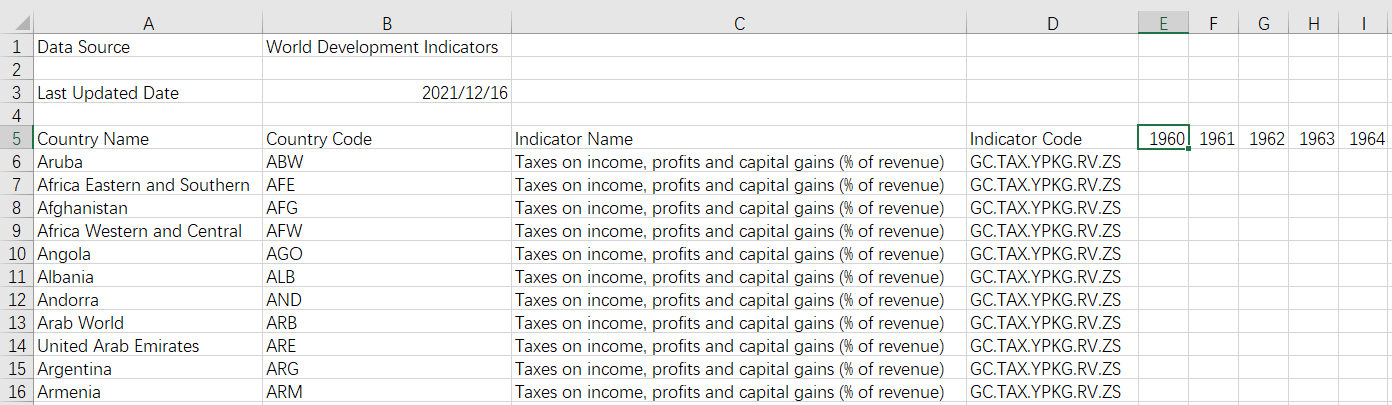
\includegraphics[width=\textwidth]{pics/001.png}
        \caption{standardize\_hor方法应用示例}
        \label{standardize_hor}
    \end{figure}

\subsection{standardize\_policy}

    \begin{lstlisting}
    standardize_policy(self, start, end, mode: str="sync", varname: str="", treat_time=0)
    \end{lstlisting}    

    这个方法适用于处理一类特殊的数据,即\textbf{政策变量}。
    
    这类变量往往连续多年取同样的值,并在个别时间节点发生变化。因此,原始数据常常仅指出了政策变化的时间节点,而没有标注每一年的变量值。\verb|standardize_policy| 方法可以将这类原始数据转化成规范的面板数据形式。

    \begin{figure}
        \centering
        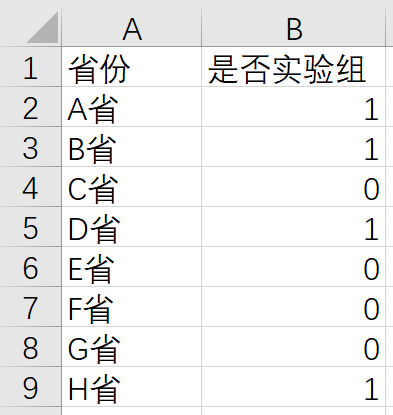
\includegraphics[height=0.15\textheight]{pics/002.png}
        \caption{同时施行的政策}
        \label{synchronic}
    \end{figure}

    \begin{figure}
        \centering
        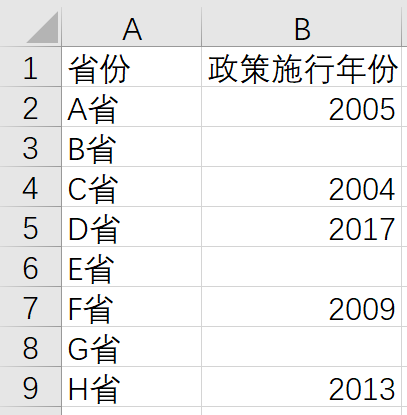
\includegraphics[height=0.15\textheight]{pics/003.png}
        \caption{不同时施行的政策}
        \label{diachronic}
    \end{figure}

    \begin{figure}
        \centering
        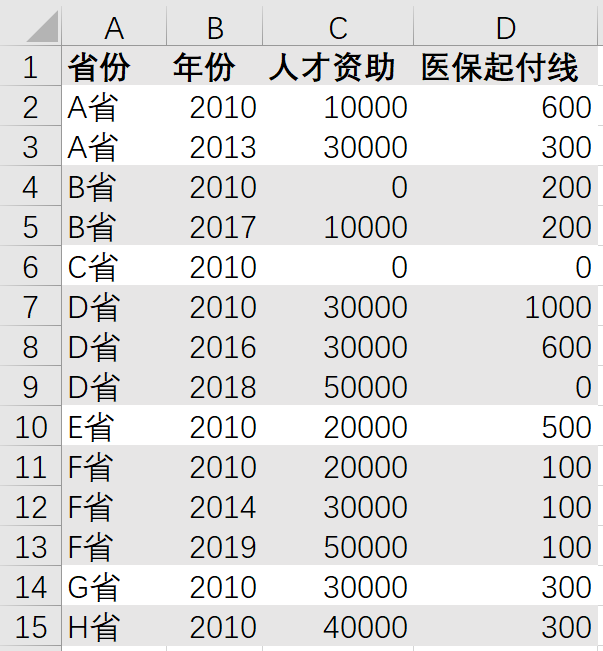
\includegraphics[height=0.25\textheight]{pics/004.png}
        \caption{多次变化的政策}
        \label{unstable}
    \end{figure}

    本方法可以处理三类原始数据:

    \begin{enumerate}
        \item \textbf{同时施行的}(synchronic)政策变量。即:控制组始终不施行政策,实验组的所有样本在同一时间施行政策。此时,传入的原始数据只需要如图\ref{synchronic}所示即可。处理这类数据时,需要在 \verb|standardize_policy()| 的参数中额外指定\textbf{政策施行年份}。
        \item \textbf{不同时施行的}(diachronic)政策变量。即:控制组始终不施行政策,实验组的样本施行政策有时间先后之别。此时,传入的原始数据只需要如图\ref{diachronic}所示即可(控制组的“政策施行年份”一列值为空)。
        \item \textbf{复杂的}(complex)政策。该模式允许原始数据中有多个变量,并且变量的值可以多次变化。此时,传入的原始数据需要如图\ref{unstable}所示(\textbf{第一列为样本名,第二列为时间,且时间必须按先后顺序排列}),明确指定每次变化的时间点,以及变化后政策变量的值。
    \end{enumerate}

    \begin{itemize}
        \item \verb|start| 参数指定面板数据从哪一个时间点开始记录。
        \item \verb|end| 参数指定面板数据在哪一个时间点结束记录。
        \item \verb|mode| 参数指定处理模式,分别对应上述的三类原始数据。值为 \verb| "sync"| 时,处理同时施行的(synchronic)政策;值为 \verb| "diac"| 时,处理不同时施行的(diachronic)政策;值为 \verb| "complex"| 时,处理复杂的(complex)政策。默认值为 \verb| "sync"|。
        \item \verb|varname| 参数指定政策变量的名称。仅在 \verb|mode="sync"| 或 \verb|mode="diac"| 时适用。
        \item \verb|treat_time| 参数指定政策(同时)施行的时间点。默认值为0。仅在 \verb|mode="sync"| 时适用。
    \end{itemize}

    注意:在所有模式中,变量值的变化在\textbf{政策施行当年}即发生。

\subsection{standardize\_ver}

    \begin{lstlisting}
    standardize_ver(self, index_row: int=0, unit_col: int=0, time_col: int=1, first_var_col: int=2)
    \end{lstlisting}    

    适用于\textbf{样本名和时间线纵向排列、变量名横向排列}的原始数据。这种排列方式基本符合MagicPanel的格式规范。\verb|standardize_ver| 方法对这种格式的数据进行一些微调,如删除多余的行和列等。

    返回值是更新内容后的一个QuasiPanel的实例。

    \begin{itemize}
        \item \verb|index_row| 参数指定索引行(即“表头”)的行号,行号从0开始计。默认值为0。计算时,空行也包括在内。经过Excel渲染的csv文件,显示的行号可能不是真实的行号;因此,最好是在记事本中打开csv文件,查看表头的行号。
        \item \verb|unit_col| 参数指定样本名称(如“国家名”“城市名”等)所在列的列号,列号从0开始计。默认值为0。计算时,空列也包括在内。
        \item \verb|time_col| 参数指定变量名称所在列的列号,列号从0开始计。默认值为1。计算时,空列也包括在内。
        \item \verb|first_var_col| 参数指定第一个变量所在列的列号,列号从0开始计。默认值为2。计算时,空列也包括在内。
    \end{itemize}

\section{Panel类方法详解}

\subsection{absorb}

    \begin{lstlisting}
    absorb(self, new_panel: "Panel", mode: str="new", mapping: dict={})
    \end{lstlisting}    

    将一个新的面板数据合并到原来的面板中。

    注意:合并时以原来的面板数据为基础。合并后保持原面板数据的样本顺序;\textbf{当新面板中有原面板没有的样本(如原面板时间只到2010年为止,但新面板存在2011年的数据)时,新面板中多出来的样本会被舍弃。}

    \verb|absorb| 方法提供两种模式:

    \begin{itemize}
        \item \textbf{新数据(new)模式},即合并一个新的数据库进来,添加为新的变量。
        \item \textbf{补充数据(complementary)模式},即用新的数据填补原有数据中的缺失值(如果不是缺失值,则不会填充,而是保留原有数据)。
    \end{itemize}

    \textbf{应慎用“补充数据模式”},因为不同来源的数据很可能有单位不一致、统计口径有差异等问题,贸然合并会影响数据质量。

    \begin{itemize}
        \item \verb|new_panel| 参数指定新的面板,需要传入一个Panel类的实例。
        \item \verb|mode| 参数指定合并的模式:\verb|"new"| 为新数据模式,\verb|"complementary"| 为补充数据模式。默认值为 \verb|"new"|。
        \item \verb|mapping| 参数指定补充数据模式中变量名的对应情况。对于新数据来说,只有在 \verb|mapping| 中指定的变量会用于数据合并,其他的变量将被忽略。\textbf{在补充数据模式下,必须一一指明变量名的对应情况,即使原变量名和对应的变量名相同。}传入数据的格式为:\verb|{"原变量名A": "对应变量名A", "原变量名B": "对应变量名B", ...}|。
    \end{itemize}

\subsection{add\_var}

    \begin{lstlisting}
    add_var(self, varname: str)
    \end{lstlisting}    

    给数据库添加一个新变量,变量的初始值为空字符串。

    \begin{itemize}
        \item \verb|varname| 参数指定新变量的名称。
    \end{itemize}

\subsection{change}

    \begin{lstlisting}
    change(self, unit: str, timepoint, var: str, value: str)
    \end{lstlisting}    

    通过指定样本名、时间点和变量名确定单元格,并改写该单元格的值。

    如果找不到对应的单元格,则不对数据作任何改动。

    \begin{itemize}
        \item \verb|unit| 参数指定样本名(如具体国家名)。
        \item \verb|timepoint| 参数指定时间点(如具体年份)。
        \item \verb|var| 参数指定变量名。
        \item \verb|value| 参数指定为该单元格赋的新值。
    \end{itemize}

\subsection{contents}

    \begin{lstlisting}
    contents(self)
    \end{lstlisting}    

    返回值为面板的当前内容。返回值的数据类型是list。

\subsection{extract}

    \begin{lstlisting}
    extract(self, varlist: list)
    \end{lstlisting}    

    通过指定变量,提取当前数据集的子数据集。返回值为Panel类的一个实例。

    如果指定的变量中有原数据集中不存在的变量,则忽略之。

    \begin{itemize}
        \item \verb|varlist| 参数指定需要提取的变量名(表的前两列无需指定)。
    \end{itemize}

\subsection{export}

    \begin{lstlisting}
    export(self, path: str, filename: str, encoding: str="utf-8")
    \end{lstlisting}    

    将当前面板数据导出为csv文件。

    \begin{itemize}
        \item \verb|path| 参数指定导出文件所在的文件夹。
        \item \verb|filename| 参数指定文件名(不含后缀“.csv”)。
        \item \verb|encoding| 参数指定csv文件的编码,默认为utf-8格式。如果使用Excel打开导出文件时乱码,可以尝试声明 \verb|encoding="gb18030"|。
    \end{itemize}

\subsection{get}

    \begin{lstlisting}
    get(self, unit: str, timepoint, var: str)
    \end{lstlisting}    

    通过指定样本名、时间点和变量名,获取面板数据中的一个单元格的值。
    
    返回值为一个字符串,即要查找的单元格的值。

    如果找不到对应的单元格,则返回\verb|None|。

    \begin{itemize}
        \item \verb|unit| 参数指定样本名(如具体国家名)。
        \item \verb|timepoint| 参数指定时间点(如具体年份)。
        \item \verb|var| 参数指定变量名。
    \end{itemize}

\subsection{get\_syn\_from\_csv}

    \begin{lstlisting}
    get_syn_from_csv(path: str, filename: str, encoding: str="utf-8")
    \end{lstlisting}    

    从csv文件中获取同义词词典。返回值为一个字典。
    
    关于该字典的形式和用途,参见\nameref{paraphrase}。

    \begin{itemize}
        \item \verb|path| 参数指定csv文件所在的文件夹。
        \item \verb|filename| 参数指定文件名(不含后缀“.csv”)。
        \item \verb|encoding| 参数指定csv文件的编码,默认为utf-8格式。
    \end{itemize}

\subsection{get\_var\_col}

    \begin{lstlisting}
    get_var_col(self, varname: str)
    \end{lstlisting}

    返回值为变量名对应的列号。
    
    如果数据中有重复的变量名(这种情况应尽量避免),则返回第一个匹配到的列号。如果找不到该变量,则返回 \verb|None|。

    \begin{itemize}
        \item \verb|varname| 参数指定要查找的变量名。
    \end{itemize}

\subsection{locate}

    \begin{lstlisting}
    locate(self, unit: str, timepoint, var: str)
    \end{lstlisting}    

    通过指定样本名、时间点和变量名,锁定面板数据中的一个单元格。
    
    返回值为一个元组,包含要查找的单元格的行号和列号(行号和列号从0开始计)。

    如果找不到对应的单元格,则返回\verb|(None, None)|。

    \begin{itemize}
        \item \verb|unit| 参数指定样本名(如具体国家名)。
        \item \verb|timepoint| 参数指定时间点(如具体年份)。
        \item \verb|var| 参数指定变量名。
    \end{itemize}

\subsection{paraphrase\label{paraphrase}}

    \begin{lstlisting}
    paraphrase(self, synonyms: dict)
    \end{lstlisting}    

    该方法可以解决一个常见的问题,即不同的数据库对同一个样本采用不同的称呼方式。如“Cambodia”和“Kampuchea”都是指柬埔寨、“Cote d'Ivoire”和“Ivory Coast”都是指科特迪瓦等。

    \begin{itemize}
        \item \verb|synonyms| 参数指定一个同义词词典。这个词典需要逐个指明每个样本的别名对应的标准名称。传入数据的格式为:\verb|{"别名1": "标准名1", "别名2": "标准名2", ...}|。
    \end{itemize}

\subsection{sort}

    \begin{lstlisting}
    sort(self, varlist: list=[], reverse=False)
    \end{lstlisting}

    将面板数据重新排序。先按照用户设置排序,对于按照用户设置无法分出顺序的,按照样本名称和时间升序排列。

    \begin{itemize}
        \item \verb|varlist| 参数指定排序依据的变量。放在前面的变量优先级更高。默认值为空列表。当 \verb|varlist| 参数为默认值时,即对原始数据按照样本名称和时间升序排列。
        \item \verb|reverse| 参数指定是否降序排列。默认值为  \verb|False|。
    \end{itemize} 

    在Python中,字符串排序是按照字典顺序,因此会出现 \verb|"345" > "1234"| 的情况。为了避免这种情况,对于所有数字型的变量,MagicPanel会将其自动转成浮点数(float)再进行排序。

\subsection{time}

    \begin{lstlisting}
    time(self)
    \end{lstlisting}    

    返回值为面板包含的所有时间点(如所有年份),从小到大排序。

\subsection{units}

    \begin{lstlisting}
    units(self)
    \end{lstlisting}    

    返回值为面板包含的所有样本名(如所有国家名),按字母顺序排序。

\subsection{variables}

    \begin{lstlisting}
    variables(self)
    \end{lstlisting}    

    返回值为面板包含的所有变量名(即“表头”的各项),按原始顺序排序。

\section{示例代码\label{example}}

您可以点击\href{https://github.com/PKU-Zyf/MagicPanel/blob/main/example.py}{此处}下载下列示例的源代码。

\begin{lstlisting}
    # 以下为MagicPanel库的示例代码。
    # 访问 https://github.com/pku-zyf/MagicPanel/,可在“example-data”文件夹获取本示例代码用到的原始数据。
    # 将“example-data”文件夹复制到本示例代码所在的路径,即可运行。
    # 所有数据仅供示例使用,无任何实际意义。

    import MagicPanel
    from os.path import dirname, join, realpath

    def main():
        # 获取原始数据所在路径。
        path = join(dirname(realpath(__file__)), "example-data")
        # 导入“人均GDP”数据(横向)。
        pn1 = (
            MagicPanel
            .QuasiPanel()
            .import_from_csv(path=path, filename="gdppc-horizonal-gbk", encoding="gb18030")
            .standardize_hor(index_row=0, unit_col=0, var_col=1, first_time_col=2)
            .gen_panel()
        )
        # 导入“人口”数据(纵向)。
        pn2 = (
            MagicPanel
            .QuasiPanel()
            .import_from_csv(path=path, filename="pop-vertical-utf8", encoding="utf8")
            .standardize_ver(index_row=2, unit_col=0, time_col=1, first_var_col=2)
            .gen_panel()
        )
        # 导入“人才政策”数据(虚拟变量)。
        pn3 = (
            MagicPanel
            .QuasiPanel()
            .import_from_csv(path=path, filename="policy-big5", encoding="big5")
            .standardize_policy(varname="人才政策", start=2011, end=2020, mode="diac")
            .gen_panel()
        )
        # 导入“专利数量”数据(横向)。
        pn4 = (
            MagicPanel
            .QuasiPanel()
            .import_from_csv(path=path, filename="patent-horizonal-gbk", encoding="gbk")
            .standardize_hor(index_row=1, unit_col=0, var_col=None, var_name="专利数量", first_time_col=1)
            .gen_panel()
        )
        # 导入“专利数量”补充数据(横向)。
        pn5 = (
            MagicPanel
            .QuasiPanel()
            .import_from_csv(path=path, filename="patent-horizonal-sup-gbk", encoding="gbk")
            .standardize_hor(index_row=1, unit_col=0, var_col=None, var_name="专利数量", first_time_col=1)
            .gen_panel()
        )    
        # 合并数据。
        pn = (
            pn1
            .absorb(pn2)
            .absorb(pn3)
            .absorb(pn4)
            .absorb(pn5, mode="complementary", mapping={"专利数量": "专利数量"})
            .sort()
        )
        # 导出数据。导出为gb18030格式,可在Windows系统的Excel中直接打开。
        pn.export(path=path, filename="result", encoding="gb18030")

    if __name__ == "__main__":
        main()
\end{lstlisting}

\end{document}
